\chapter{Introduction}
\label{ch:intro}

This chapter addresses the main concepts of \gls{rl} and why \gls{rl} has become more popular.
In section \ref{sec:intro-approaches}, some important differences in the possible approaches for solving \gls{rl} problems are highlighted.
Afterwards, some of the classical \gls{rl} problems that are solved to benchmark new state-of-the-art algorithms are introduced.
Finally, the feasibility of using \gls{rl} \gls{irl} is discussed.

%------------------------------------

\section{The reinforcement learning problem}
\label{sec:intro-problem}

\gls{rl} is a special type of \gls{ml} where algorithms are used to take actions in an environment.
These algorithms are often referred to as agents which should learn a policy that maps the current state of the environment ($S_t$) to an action ($A_t$) that can be taken in that state of the environment.
Upon taking an action, or after completing a series of actions, a reward ($R_t$) is given to the agent in the form of a positive or negative numerical value and the environment state may be updated.
Through repeated trial-and-error interactions, experience is collected.
This experience can then be used by the agent to learn a policy which chooses the optimal action for a given state.
According to \citet{rl_intro_handbook}, it is this trial-and-error search combined with a potentially delayed reward which distinguishes \gls{rl} from other types of \gls{ml}.
A typical \gls{rl} cycle is visualised in Figure \ref{fig:intro_rl_cycle}.

\begin{figure}[ht]
    \centering
    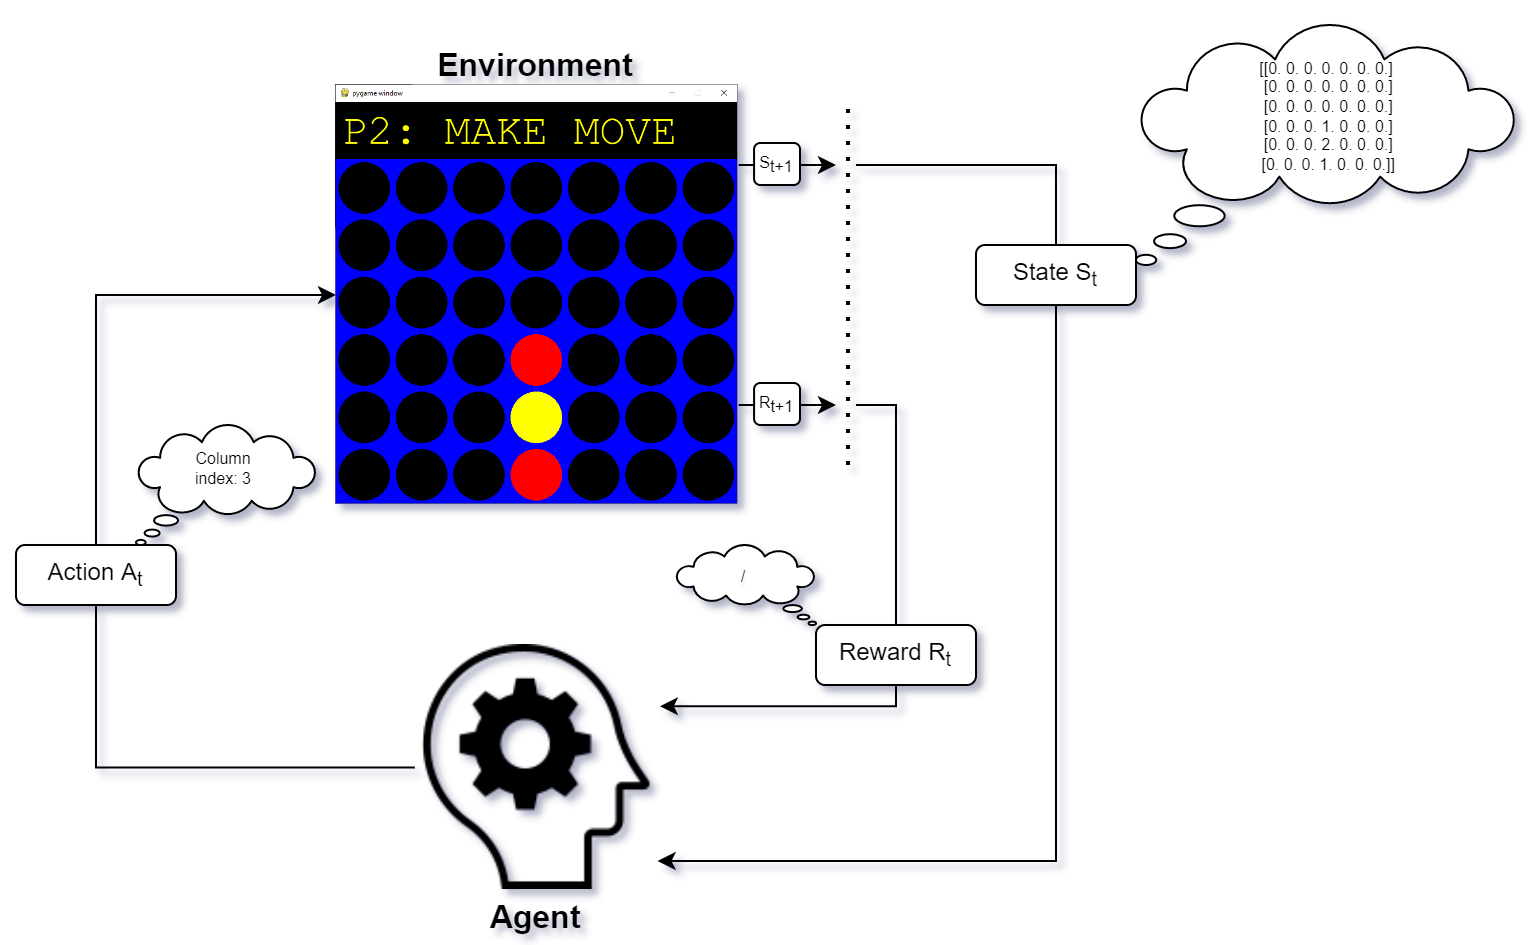
\includegraphics[width=0.9\linewidth]{images/rl_environment.png}
    \captionsetup{width=0.9\linewidth}
    \captionsetup{justification=centering}
    \caption{Typical \gls{rl} cycle annotated with examples for a single connect four game step which doesn't yield a reward.}
    \label{fig:intro_rl_cycle}
\end{figure}


Since the rewards can be considered a form of feedback given to the algorithm, these types of algorithms are not completely unsupervised.
However, classical supervised learning tasks often require far more supervision than \gls{rl}.
Consequently, \gls{rl} is often seen as a third \gls{ml} paradigm next to supervised and unsupervised learning.
Since the agent can learn in an online setting, there is also often no or minimal data needed upfront.
However, training an agent in an online manner, as to have the agent collect experience ($\approx$ data) itself, can take a considerable amount of time, even when using parallelized simulation.
It is also noted that offline \gls{rl} using pre-collected data for training exists.


As a result of not having direct instructions on what to do, it is difficult or even impossible for a \gls{rl} agent to decide if a learned policy is indeed the optimal policy.
Thus, an algorithm should be exploratory enough to evaluate many or even all possible policies over time whilst also being greedy enough so that the collected reward is being maximised according to the currently used policy.
Balancing this exploration/exploitation behaviour is one of many challenges in \gls{rl}.
A classical approach to solve this problem is by using epsilon-greedy.
In epsilon-greedy, epsilon ($\epsilon$) denotes the probability of taking a random action over the greedy action for any given step ($t$).
Finding a balance between exploration/exploitation becomes even harder when taking into account the time it can take to perform a singular step.
This means that mathematical proofs of optimal convergence for exploration strategies relying on infinite steps are even less likely to hold in real-life situations with finite time.

Whilst this definition of the \glsfirst{rl} problem remains rather abstract, it captures most of the requirements of a good \gls{rl} algorithm.
Indeed, the \gls{rl} problem is less concrete than some other problems in \gls{ml} allowing for high creativity in approaches.
Some of the many different types of approaches are discussed in section \ref{sec:intro-approaches}.
The handbook by \citet{rl_intro_handbook} gives a more detailed introduction to \gls{rl} if you have some form of computer science background.


%------------------------------------

\section{Markov Decision Process}
\label{sec:intro-mdp}

As discussed in section \ref{sec:intro-problem}, the \gls{rl} problem definition is rather abstract.
Whilst this allows for many types of solutions to be created, having a more formal representation of the \gls{rl} problem can be desired.
This is especially handy for mathematical reasoning over \gls{rl} and proving certain properties of a \gls{rl} algorithm.
To facilitate this need, \glspl{mdp} are often used as a mathematically idealized form of the \gls{rl} problem with specific properties.
Equation \ref{eq:intro_mdp} gives the mathematical definition of a \gls{mdp}.

\begin{equation}
\begin{aligned}
\text{MDP} &= \langle S, A, R, \gamma, p \rangle
\\
S &= \text{A set of states}
\\
A &= \text{A set of actions}
\\
R &= \text{A set of rewards}
\\
\gamma &= \text{A discount factor, } \gamma \in [0.1]
\\
p &= \text{A transition function which desribes the dynamics}
\end{aligned}
\label{eq:intro_mdp}
\end{equation}

Comparing the formal definition of an \gls{mdp} to the typical \gls{rl} cycle shown in Figure \ref{fig:intro_rl_cycle}, it becomes apparent that many of the \gls{rl} problems can indeed be formulated as a \gls{mdp}.
Many variants of \glspl{mdp} exist, with many of them often assuming certain properties such as the Markov property.
Intuitively, the Markov property means that the transition from the current state to the next state is only dependent on the current state and not on any of the previous states the agent was in.
For the annotated connect four example in Figure \ref{fig:intro_rl_cycle}, the Markov property holds.
Indeed, all aspects of the past agent-environment interaction that make a difference in the future are captured in the current state which is simply a representation of the board.
Intuitively, when neglecting potential human bias towards certain columns that could be learned, it doesn't matter how to current board emerged in deciding an optimal next move.
\citet{rl_intro_handbook} go over the Markov property and other properties that are often assumed for \glspl{mdp} in more detail.

As typical \gls{rl} problems can be represented as \glspl{mdp}, trying to solve \glspl{mdp} corresponds to solving the formalised \gls{rl} problems. Solving a \gls{mdp} corresponds to acting in the \gls{mdp} such that the expected discounted return is maximized.
The expected discounted return is given in Equation \ref{eq:intro_expected_discounted_return}.
From this equation, it becomes visible how important it is to choose a good discount factor since a low $\gamma$ will result in a \textit{myopic agent} ($\approx$ greedy) and a high $\gamma$ will result in a \textit{farsighted agent} ($\approx$ exploratory).
As a result, not only the reward influences the goal of a \gls{rl} agent but also the discount factor ($\gamma$).
It is noted that for some situations the discount factor can be 1, resulting in a special type of expected return: the undiscounted expected return.

\begin{equation}
G_t = R_{t+1} + \gamma R_{t+2} + \gamma^2 R_{t+3} + ... = \sum_{k=0}^{\infty}{\gamma^k R_{t+k+1}}
\label{eq:intro_expected_discounted_return}
\end{equation}


%------------------------------------

\section{Reinforcement learning is becoming more popular}
\label{sec:intro-popular}

The term \gls{ai} is used in conventional media a lot, even for systems that shouldn't be classified as \gls{ai}.
In contrast, terms like \gls{ml} are far less known by the wider public, let alone the term \gls{rl}.
However, the computer program that beat a world champion Go player is likely one of the most recent achievements of \gls{ai} the wider public will remember.
Indeed, with $\approx 10^{360}$ possible game states for the Go game, far bigger than $\approx 10^{123}$ for chess, the AlphaGo system by \citet{alphago} that beat a world champion Go player was a monumental milestone.
This AlphaGo system is a popular example of \gls{rl}, although the use of human and domain knowledge combined with provided known rules makes AlphaGo a non-pure form of \gls{rl}.
Follow up versions such as AlphaGo Zero \citep{alphago_zero}, AlphaZero \citep{alphazero} and MuZero \citep{muzero} focused on removing these extra dependencies from the algorithm, making them a purer form of \gls{rl} whilst also having better and more general performance. 

All of the above systems were created by DeepMind, a Google-owned company.
As the name of the company suggests, all of these systems combine \gls{dl} with \gls{rl} to create a special type of \gls{rl} often referred to as \gls{drl}.
Whilst \gls{dl} was revolutionising for many fields in \gls{ml}, it was especially groundbreaking in \gls{rl} research.
Indeed, whilst \gls{rl} has decades' worth of research coming from multiple almost independent threads of history \citep[Section 1.6]{rl_intro_handbook}, it was only with the introduction of \gls{drl} that the field has received high coverage in major publications journals such as Nature \citep{rl_intro_handbook, alphago, alphago_zero, dqn}.
Section \ref{sec:intro-approaches} explains in more detail why \gls{drl} is so powerful and how it opened many new doors for the \gls{rl} field.

When looking at the most impressive \gls{rl}-based systems, it becomes apparent that big companies and institutions such as DeepMind and OpenAI are responsible for the majority of these works.
Even state-of-the-art algorithms such as Rainbow by \citet[DeepMind]{rainbow} and famous libraries such as the Gym library by \citet[OpenAI]{gym} often originate from these bigger companies.
For newcomers first learning about \gls{rl} this may seem intimidating and raise the idea that \gls{rl} requires a lot of resources to create meaningful systems.
Whilst many examples can be given of extensions to existing algorithms and many libraries exist which are provided by smaller institutions or even individuals, complete systems from such smaller institutions with obvious real-life applications are harder to find.
Section \ref{sec:intro-irl} discusses the feasibility of developing such complete systems in more detail.

%------------------------------------

\section{Common approaches for reinforcement learning}
\label{sec:intro-approaches}
% e.g. tabular, mdp, dl, ... (model free etc)
% Maar ook DQN en Rainbow

As discussed in section \ref{sec:intro-popular}, \gls{drl} has opened many new doors for the \gls{rl} field, but many more different approaches for \gls{rl} exist.
A first big division can be made on so called model-based and model-free approaches.
This differentiation relates to whether or not the algorithm requires a \textit{perfect model}.
Such a perfect model should give exact probabilities and information about all possible state-action pairs for an environment.
Whilst often used for proving theoretical aspects of \gls{rl} through \gls{dp}, these types of approaches don't have many other use cases.
This is in part because such a perfect model is in contrast with the ideology of \gls{rl} using delayed rewards.
More importantly, providing a perfect model has been proven to be computationally too hard or even impossible in most cases.
Contrary to what the name suggests, model-free approaches still require a model.
However, the model should only be able to generate experiences and thus fits in more easily with delayed rewards and is possible to be made in many more scenarios.
Take for example the simple game of connect four, a model that generates experiences by recognising a win, a loss or a tie is simple, allowing for model-free approaches.
Defining probabilities of each of these outcomes at any given state for any given action can become hard very fast, making model-based approaches impractical, if not impossible.
Section \ref{sec:connect_four_rl-harder_then_you_think} explains how connect four has over \textit{four trillion} possible board layouts ($\approx 10^{13}$), further illustrating how hard providing a perfect model can be.

Another major differentiation that is made between \gls{rl} algorithms is whether the algorithm is on-policy or off-policy.
As discussed in section \ref{sec:intro-problem}, the goal of an agent in \gls{rl} is to learn a policy which chooses an action for any given state.
This policy to be learned by the agent is called the \textit{target policy}.
This target policy is thus often the optimal policy, as we want the agent to learn to behave perfectly optimal in an environment.
However, for an agent to ensure that it is using the optimal policy, sufficient exploration of all possible policies should be done as was already discussed in section \ref{sec:intro-problem}.
Due to this balancing, a conflict of interest arises.
The requested agent's target policy is the optimal policy, but to ensure this, the agent has to remain exploratory causing it to never behave optimally the whole time.
Whilst strategies such as epsilon-decay exist, where the exploration is reduced over time to limit divergence from the optimal policy, these strategies are not always ideal.
What is essentially wanted is that the agent has a notion of two policies.
A \textit{target policy} which should be learned, e.g. the optimal policy, and a \textit{behaviour policy} to collect experience, e.g. the learned target policy that takes random actions systematically.
The relation between these two policies is what defines an algorithm to be on-policy or off-policy.
Off-policy indicates that both policies are different whilst on-policy indicates both policies are equal.
On-policy approaches can thus be seen as a special type of off-policy approaches.


A last important notion for this paper is \glsfirst{drl} approaches and how they differ from tabular approaches.
The main rationale behind tabular approaches is to maintain a big table of all possible states and the actions that can be taken in that state and associate a metric value to each such pair.
For example, each state-action pair might have an expected reward associated with it.
Choosing the action with the highest expected reward then boils down to choosing that state-action pair with the highest value and learning from experience consists of updating that table.
Whilst this can be very powerful for low complexity environments, it can quickly blow up in more complex environments.
Section \ref{sec:connect_four_rl-harder_then_you_think} discusses how making such a table for the relatively simple game of connect four can quickly become non-tractable.
\Gls{drl} doesn't maintain such a table but rather fits a deep learning model on the state and predicts actions from it.
This directly shows how \gls{drl} enables far more use-cases for \gls{rl}.
Since \gls{dl} is known to be great at reducing high-dimensional data such as images to low-dimensional features, it can also be faster to train for more complex environments that may still be viable to learn through tabular methods, although this is not always the case.
\Gls{rl} algorithms could be even further categorised based on other criteria and whilst these different categorisations are important, they fall outside the scope of this paper.


%------------------------------------

\section{Classical reinforcement learning problems}
\label{sec:intro-classical_rl}
% gym etc

A complete \glsfirst{rl} system consists of three main components: a conversion mechanism from an environment state to a computer representation of that state, a \gls{rl} algorithm that maps that environment state to an action and a component responsible for executing the chosen action.
In a real life environment system, these three different components often require a multi-disciplinary team to be implemented.
Take for example a \gls{rl} based robot lawn mower.
To convert the environment to a computer representation, cameras and other sensors could be used to create a mapping of the environment.
This requires expertise from computer vision and other fields to enforce the robot doesn't drive into pools or other forbidden areas, as we don't want to needlessly destroy these products by letting the \gls{rl} algorithm learn it shouldn't drive into pools.
The implementation of the \gls{rl} algorithm itself requires a specialist in \gls{rl}.
Finally, to perform the suggested action by the algorithm, a robotics engineer might be needed to control such a robot.
Whilst some of these requirements could be loosened by re-using existing systems and \glsfirst{drl} can work directly on captured images, it becomes clear that implementing a complete \gls{rl} system requires more than just \gls{rl} expertise.

This is one of the reasons academic research focusing on \gls{rl} algorithms often make use of simulated environments to limit the focus only on the \gls{rl} algorithm component.
This lowers the entry boundary compared to a complete \gls{rl} system and enables smaller teams or even individuals to contribute to the \gls{rl} field by focusing solely on the \gls{rl} component.  
Another bonus of simulation is that it is often far faster to complete a step in the environment than a real-life system would take, allowing for far faster learning.
Some simulated environments and algorithms even allow for running training in parallel, making the often notoriously long training procedure of \gls{rl} more manageable.
These simulated environments are often games, since the winning criteria of a game are often easy to define but providing exact probabilities for each state is often computationally too hard or even impossible, fitting in perfectly with the delayed reward ideology of \gls{rl} discussed in section \ref{sec:intro-problem}.

Many libraries that provide simulated game environments exist.
This allows the creator of a \gls{rl} algorithm to easily test the performance on a wide variety of games and since these games are often identical between papers, it allows for easy comparison between algorithms as well.
Perhaps the most common simulated environments are Atari 2600 games.
The Atari 2600 is a gaming console from the late 70's known for its games with relatively simple rules and winning/losing conditions such as Pong and Breakout.
Many frameworks exist that provide some of the most popular Atari 2600 games with specific support for \gls{rl}.
The Gym library for Python by \citet[OpenAI]{gym} is one of the most popular.
Most of these frameworks, including the Gym library, are based on Stella which is an Atari 2600 emulator by \citet{stella}.
Whilst Gym is one of the most popular environment providing libraries and many Python libraries exist that provide implementations of the most common \gls{rl} algorithms with Gym support, it should be noted Python isn't the most efficient programming language which isn't ideal in combination with the already long training times that \gls{rl} algorithms often require.
Because of this, the Arcade Learning Environment (ALE) with both C++ and Python support for Atari 2600 games by \citet{ale} is also a very popular choice in literature among many others.

Since this paper focuses on the feasibility of using a \gls{rl} algorithm as a computer opponent in indie games, we focus on Gym-like environments in Python.
This is by far the combination of programming language and environment style that has the most available \gls{rl} libraries, making implementation of common \gls{rl} algorithms quicker and easier, perhaps at the cost of computational efficiency.
Since the Gym environment focuses on providing single agent \gls{rl} environments, it does not have a standard for defining multi-agent environments in which this paper is interested.
Many environment libraries that support \gls{marl} have been proposed, each having there own way of representing the environments.
One of the most used libraries for providing \gls{marl} environments is the Petting Zoo one by \citet{pettingzoo}.
The general interaction methods of Petting Zoo environments are very similar to those of the Gym environments, aiding in its popularity.
It is also one of the few \gls{marl} environment libraries that has some form of support by common \gls{rl} algorithm providing libraries such as Tianshou by \citet{tianshou} and Ray RLlib by \citet{rllib}.
Petting Zoo provides multi-agent games from the Atari 2600 amongst other classical multi-player games such as Tic-Tac-Toe and Uno.




%------------------------------------

\section{Feasibility of using reinforcement learning in real life}
\label{sec:intro-irl}
% e.g. optimalisatie van dingen etc

In section \ref{sec:intro-classical_rl}, it was discussed how a complete \gls{rl} system consists of three main components which often require a multi-disciplinary team to create.
Finding the right people for such a team is not only a hard task, but can require significant monetary resources as well.
Adding to this, the required computational power and training time of complex \gls{rl} algorithms are also an issue.
The discussed Alpha Go system by \citet{alphago} was trained for three weeks using computational power comparable to over 50 high-end graphic cards.
This first version of the Go champion beating algorithm also used a lot of domain knowledge, stepping away from the attractive aspect of \gls{rl} not strictly requiring data or great domain expertise upfront.
This required domain knowledge and computational power make the system expensive in training costs alone.
In many cases, the system will not perform as wanted from the first time either, so the expensive training procedure has to be repeated for a variety of system iterations.
It is also challenging to estimate how good \gls{rl} will be at a given task upfront, often requiring test trials to get a grasp on potential performance.
Whilst unexpected bad performance can have significant value in academic literature, the commercial value is rather limited to investing companies.
These properties combined with general challenges in \gls{rl} are part of the reason \gls{rl} hasn't seen the widespread adoption other \gls{ml} approaches have seen.
It also limits the most popular ground-breaking examples of \gls{rl} such as the Go beating algorithm to organisations with sufficient funds.
This explains in part why many of the big examples of \gls{rl} originate from the same popular companies such as OpenAI and DeepMind.

Luckily, new state-of-the-art in \gls{rl} and \gls{drl} has shown to be far more sample efficient and general.
Take for example the Rainbow algorithm by \citet{rainbow}.
In their paper, \citet{rainbow} studied six extensions to the popular \gls{dqn} algorithm and combined the strong points into a singular \gls{rl} algorithm they call Rainbow.
Not only does Rainbow significantly outperform these extensions on the Atari 2600 games which were discussed in section \ref{sec:intro-classical_rl}, it does so by requiring far fewer samples.
With the distributional DQN extension proposed by \citet{distributional_dqn} being the best out of the six extensions when tested individually, Rainbow used 7 million frames compared to 44 million frames of training required by the distributional DQN approach.
The final best-found performance of Rainbow when looking at the median human-normalized score was 223\% compared to 164\% of distributional DQN.
A recent follow-up of AlphaGo named MuZero by \citet{muzero} is also significantly faster in training and didn't require domain knowledge.
This also made the system more generalized, as shown by the EfficientZero system proposed by \citet{efficient_zero} which is based on MuZero. EfficientZero got human performance as the median for the Atari 2600 games in just two hours of what they call real-time game experience.
This shows that new state-of-the-art algorithms can reduce the above-mentioned feasibility challenges with \gls{rl} to a certain extent.

Indeed, in very recent years, more and more real-life \gls{rl} systems are being implemented and it is often assumed that \gls{rl} is still in its early days, especially for real-life applications.
Due to \gls{rl} learning rules and policies itself, it isn't used in real-world environments often where it could potentially harm its surroundings.
Rather, it is more often used for determining strategies and policies in computer specific tasks where bad output isn't catastrophic.
Popular use cases include providing personalised suggestions such as movie suggestions.
It is feasible to provide valuable features for movies and through metrics such as watch time, a reward for the provided suggestion can also be given.
Thus, having features and a delayed reward, the main ingredients for \gls{rl} are in place.
Whilst bad suggestions won't be appreciated by the end-user, it doesn't cause any real harm either.
However, \Gls{rl} has also been proven useful in scenarios where the output of the \gls{rl} algorithm can have catastrophic consequences.
Planning and strategy determination tasks are one such example.
\Citet{cooling} describe a system where \gls{rl} is used to determine a cooling strategy for data servers.
Some mechanisms are in place to ensure no overheating can occur.
\Citet{cooling} found that \gls{rl} saves significant energy required for cooling whilst the temperatures of the data-servers remained acceptable. 

Whilst these use cases are great news for more widespread adoption of \gls{rl}, these applications are often still aimed at bigger institutions with sufficient funds.
True applications for small businesses or even individuals are hard to come by in the current state of \gls{rl}.
However, since many of the commonly used environments for \gls{rl}, such as the Atari 2600 games, are gaming environments, one possible application addressing indie developers, is the use of \gls{rl} for providing more human-like computer opponents in video games.
The next chapters will address \glsfirst{marl}, a type of  \gls{rl} where two or more agents are present in an environment, as is the case with multiplayer games. The other chapters of this paper study the feasibility of \gls{rl} to be used by indie game developers for creating a human-like connect four computer opponent by implementing all required components and evaluating them. 
